


次に, 変換にある種「失敗」が起きうることも想定する. 
例えばS系の変換後の状態が欲しかった状態とはずれていたり, C系がうまく作動しなかったり, 仕事浴とのエネルギーのやり取りが思い通りにならなかったりと, 色々と考え得る. 
それも加味した上で, 「大体」変換できる, ことを次のように定式化する. 

\begin{mydfn}[$\varepsilon$-approximate Single-Shot thermodynamic process]\label{dfn.approximate_single-shot_transformable}
  $\varepsilon \geq 0$とする. 
  $\hat{\rho}_{\text{S}}$, $\hat{\rho}_{\text{S}}'$をそれぞれS系のHamiltonianが$H_{\text{S}}$, $H_{\text{S}}'$であるような状態とする. 
  $\hat{\rho}_{\text{SCW}}^G$についてのGibbs保存写像$\symcal{E}_{\text{SCW}}$が存在して, $\hat{\rho}\coloneqq \hat{\rho}_{\text{S}}\otimes\ket{0}\bra{0}\otimes\ket{E_i}\bra{E_i}$, $\hat{\rho}'\coloneqq \hat{\rho}_{\text{S}}'\otimes\ket{1}\bra{1}\otimes\ket{E_f}\bra{E_f}$とするとき, 
  \begin{equation}
    D(\symcal{E}_{\text{SCW}}(\hat{\rho}), \hat{\rho}')\leq \varepsilon
  \end{equation}
  が成立するとき, $\hat{\rho}_\text{S}$は$\hat{\rho}_\text{S}'$に$\varepsilon$-approximate $w$-assisted transformableという. 
\end{mydfn}
この定義の意味するところは, 生成した状態が積状態かも, C系やW系がうまくいったのかもわからないが, ともかく全体としては欲しかった状態の$\varepsilon$近傍にはいる状態は作れる, ということだ. 

\begin{figure}[H]
  \centering
  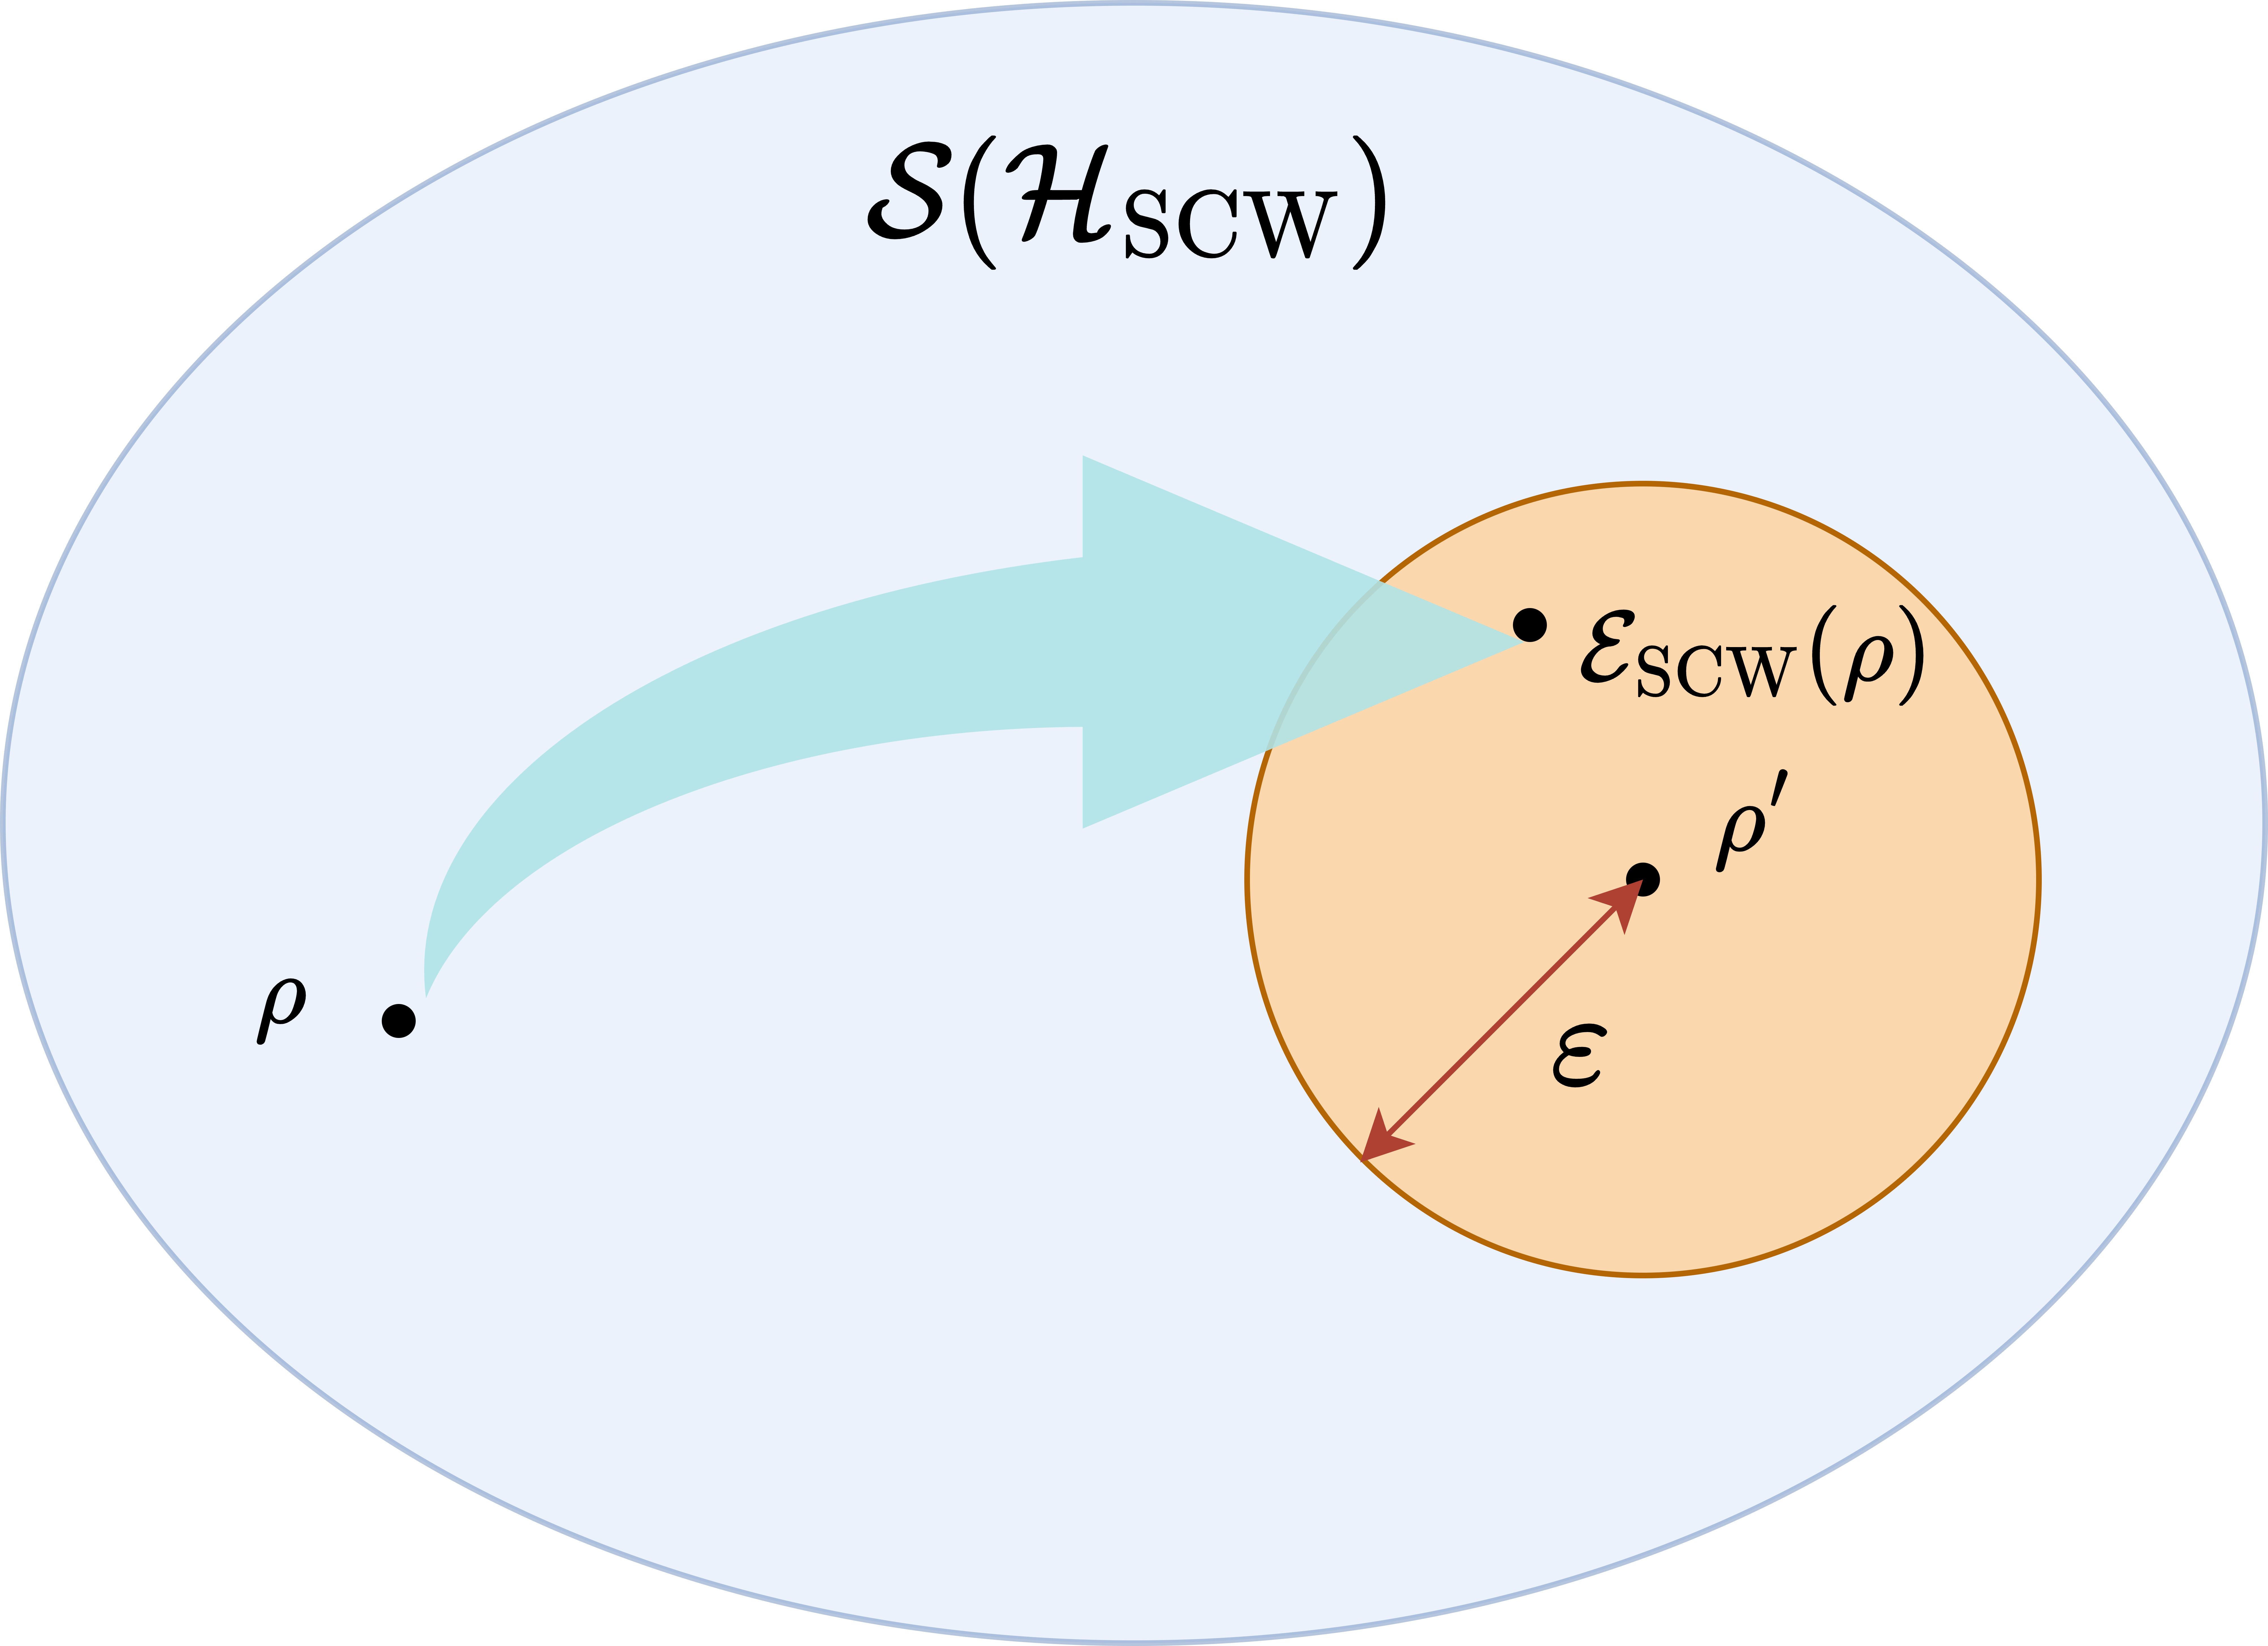
\includegraphics[keepaspectratio, scale=0.03]{images/approximate.drawio.png}
  \caption{イメージ図}\label{fig.approximate_image}
\end{figure}
それでは、できた状態のうち, S系の部分はどのくらい欲しかった$\hat{\rho}_\text{S}'$に似ているのだろうか?
次の命題より, 特にS系に絞ってみても出力された状態と欲しかった状態は$\varepsilon$近傍にあることが確認できる. 
\begin{myprop}
  $\hat{\rho}_{\text{S}}''\coloneqq \tr_{\text{CW}}[\symcal{E}_{\text{SCW}}(\rho)]$とする. 
  このとき, 
  \begin{equation}
    D(\hat{\rho}_{\text{S}}''||\hat{\rho}_{\text{S}}')\leq \varepsilon
  \end{equation}
\end{myprop}

\begin{proof}
  部分トレースはCPTP写像だったので, トレース距離の単調性(定理\ref{thm.data-processing_inequality})より
  \begin{equation}
    \varepsilon\geq D(\symcal{E}_{\text{SCW}}(\hat{\rho}), \hat{\rho}')\geq D(\tr_{\text{CW}}\circ\symcal{E}_{\text{SCW}}(\hat{\rho}), \tr_{\text{CW}}(\hat{\rho}'))=D(\hat{\rho}_{\text{S}}''||\hat{\rho}_{\text{S}}')\
  \end{equation}
  示された. 
\end{proof}

Approximate CaseにもExact Caseのときのような$\varepsilon$-approximate $w$-assisted transformableのための必要条件/十分条件を与える定理があるが, 必要条件については量子仮説検定ダイバージェンスが登場し, やや綺麗ではない
\footnote{$\varepsilon$-approximate $w$-assisted transformableの定義の条件を少し強めることでよりシンプルな形にすることができる. 
詳細は\cite{SagawaEntropy}を参照. 
定義\ref{dfn.approximate_single-shot_transformable}の利点は次のAzssymptotic Caseにうまく接続できる点にある. }. 
十分条件の方には平滑化ダイバージェンスが登場し, 良い形をしている. 

\begin{mythm}\label{thm.approximate-case_single-shot_work_bounds}
  $\hat{\rho}_{\text{S}}$, $\hat{\rho}_{\text{S}}'$をそれぞれS系のHamiltonianが$H_{\text{S}}$, $H_{\text{S}}'$であるような状態とする. 
  $\varepsilon\geq 0$とする. 
  \begin{enumerate}
    \item[(a)](必要条件): $\hat{\rho}_\text{S}$は$\hat{\rho}_\text{S}'$に$\varepsilon$-approximate $w$-assisted transformableならば, $0<\eta<1-\varepsilon$において
    \begin{equation}
      \beta(w-\Delta F_{\text{S}})\geq S_{\text{H}}^{\eta+\varepsilon} (\hat{\rho}_{\text{S}}{}'||\hat{\rho}_{\text{S}}^{G}{}')-S_{\text{H}}^\eta (\hat{\rho}_{\text{S}}||\hat{\rho}_{\text{S}}^G)-\ln\left( \frac{\eta+\varepsilon}{\eta} \right)
    \end{equation}
    が成立. 
    \item[(b)](十分条件): $\hat{\rho}_{\text{S}}$, $\hat{\rho}_{\text{S}}'$について
    \begin{equation}
      \beta(w-\Delta F_{\text{S}})\geq S_{\infty}^{\varepsilon/2} (\hat{\rho}_{\text{S}}{}'||\hat{\rho}_{\text{S}}^{G}{}')-S_{0}^{\varepsilon/2}  (\hat{\rho}_{\text{S}}||\hat{\rho}_{\text{S}}^G)
    \end{equation}
    ならば, $\hat{\rho}_\text{S}$は$\hat{\rho}_\text{S}'$に$\varepsilon$-approximate $w$-assisted transformableである. 
  \end{enumerate}
\end{mythm}

\begin{proof}
  \cite{SagawaEntropy}を参照. 
\end{proof}





